% The audit pipeline with real rasters, in two rows so that it reads at README width: Sentinel-2 bands in, frozen
% encoder (narrowing) and head (widening), prediction / confidence / boundary layers; then the review set at a 5%
% budget (boundary first) drawn on the scene, the reasons per window, the reviewer; the second row runs right to
% left under the outputs, so the whole figure is one snake. Scene: okavango_80 (exp11, exp37).
% Build: pdflatex audit_pipeline.tex; export: osascript -l JavaScript pdf2png.js audit_pipeline.pdf ../audit_pipeline.png 3000
\documentclass[tikz,border=3mm]{standalone}
% Shared style for the diagrams: layered slanted rasters with shadows, geometric model parts, few words.
\usepackage{graphicx}
\pagecolor{white}   % an explicit page background: transparent pages export as black in some rasterisers
\usetikzlibrary{positioning,arrows.meta,shadows,shapes.geometric,calc,fit,backgrounds}
\definecolor{ink}{HTML}{1F2937}
\definecolor{muted}{HTML}{6B7280}
\definecolor{oeteal}{HTML}{0F766E}
\definecolor{oeamber}{HTML}{D97706}
\definecolor{oeviolet}{HTML}{6D28D9}
\definecolor{oeblue}{HTML}{2563EB}
\definecolor{oered}{HTML}{DC2626}
\newlength{\rw}\setlength{\rw}{2.3cm}   % raster width on the page (before the slant)
\tikzset{
  >=Stealth, font=\small,
  plane/.style={inner sep=0pt, outer sep=0pt, transform shape, yscale=0.55, yslant=0.35, draw=ink!60, line width=0.4pt,
                drop shadow={shadow xshift=0.7mm, shadow yshift=-0.7mm, opacity=0.25}},
  flat/.style={inner sep=0pt, outer sep=0pt, draw=ink!60, line width=0.4pt, drop shadow={shadow xshift=0.7mm, shadow yshift=-0.7mm, opacity=0.25}},
  lab/.style={font=\scriptsize, text=ink, inner sep=1pt, align=center},
  sub/.style={font=\scriptsize, text=muted, inner sep=1pt, align=center},
  part/.style={draw=ink, line width=0.6pt, drop shadow={shadow xshift=0.8mm, shadow yshift=-0.8mm, opacity=0.3}},
  card/.style={draw=ink!70, fill=white, rounded corners=2pt, line width=0.5pt, inner sep=4pt, drop shadow={shadow xshift=0.8mm, shadow yshift=-0.8mm, opacity=0.25}},
  flow/.style={->, line width=0.9pt, draw=ink},
  cell/.style={draw=oeamber, line width=0.9pt, fill=none},
  errcell/.style={draw=oered, line width=0.6pt, fill=none},
}
% \raster{name}{x}{y}{file}: one slanted raster plane centred at (x, y)
\newcommand{\raster}[4]{\node[plane] (#1) at (#2,#3) {\includegraphics[width=\rw]{rasters/#4}};}
% \flatraster{name}{x}{y}{file}{width}: an unslanted raster
\newcommand{\flatraster}[5]{\node[flat] (#1) at (#2,#3) {\includegraphics[width=#5]{rasters/#4}};}
% \cells{plane node}{grid size}{style}{list macro}: outline windows r/c of a G x G grid on a slanted plane
\newcommand{\cells}[4]{%
  \begin{scope}[shift={(#1.center)}, yscale=0.55, yslant=0.35]
    \pgfmathsetlengthmacro{\cw}{\rw/#2}
    \foreach \r/\c in #4 {
      \draw[#3] ({(\c-#2/2)*\cw}, {(#2/2-\r-1)*\cw}) rectangle ++(\cw, \cw);
    }
  \end{scope}}
% same on a flat raster of width #5
\newcommand{\flatcells}[5]{%
  \begin{scope}[shift={(#1.center)}]
    \pgfmathsetlengthmacro{\cw}{#5/#2}
    \foreach \r/\c in #4 {
      \draw[#3] ({(\c-#2/2)*\cw}, {(#2/2-\r-1)*\cw}) rectangle ++(\cw, \cw);
    }
  \end{scope}}
% three-plane stack: \stack{prefix}{x}{y}{back}{mid}{front}
\newcommand{\stack}[6]{\raster{#1back}{#2}{#3}{#4}\raster{#1mid}{#2+0.15}{#3+0.75}{#5}\raster{#1}{#2+0.3}{#3+1.5}{#6}}
% Encoder and decoder are trapezoids in opposite directions (rule from the user, 2026-09-08):
% \encoderShape{name}{x}{y}{width}{height}{fill}: wide at the left, narrow at the right (in -> compressed)
% \decoderShape{name}{x}{y}{width}{height}{fill}: narrow at the left, wide at the right (compressed -> out)
\newcommand{\encoderShape}[6]{%
  \draw[part, fill=#6] (#2,#3-#5/2) -- (#2,#3+#5/2) -- (#2+#4,#3+#5/4) -- (#2+#4,#3-#5/4) -- cycle;
  \coordinate (#1) at (#2+#4/2,#3); \coordinate (#1in) at (#2,#3); \coordinate (#1out) at (#2+#4,#3);}
\newcommand{\decoderShape}[6]{%
  \draw[part, fill=#6] (#2,#3-#5/4) -- (#2,#3+#5/4) -- (#2+#4,#3+#5/2) -- (#2+#4,#3-#5/2) -- cycle;
  \coordinate (#1) at (#2+#4/2,#3); \coordinate (#1in) at (#2,#3); \coordinate (#1out) at (#2+#4,#3);}

\def\sceneReview{0/10, 0/11, 0/29, 1/22, 1/30, 3/25, 4/9, 6/8, 8/9, 8/11, 9/9, 9/12, 10/11, 10/14, 11/15, 13/16, 15/15, 16/15, 16/17, 19/16, 19/23, 20/19, 20/22, 22/14, 22/15, 22/16, 23/14, 23/19, 24/15, 25/14, 25/15, 25/16, 25/17, 25/21, 25/31, 26/16, 26/17, 26/30, 27/22, 27/23, 27/30, 28/22, 28/23, 28/31, 29/21, 29/22, 30/20, 30/21, 30/22, 31/19, 31/21}
   % defines \sceneReview as a r/c list
\setlength{\rw}{2.7cm}
\tikzset{lab/.style={font=\small, text=ink, inner sep=1pt, align=center},
         sub/.style={font=\footnotesize, text=muted, inner sep=1pt, align=center}}
\begin{document}
\begin{tikzpicture}
  % ================= row 1: input -> encoder -> head -> outputs
  \stack{in}{0}{5.0}{scene_b11.png}{scene_b08.png}{scene_rgb.png}
  \node[sub, anchor=west] at ($(in.east)+(0.12,0)$) {RGB};
  \node[sub, anchor=west] at ($(inmid.east)+(0.12,0)$) {NIR};
  \node[sub, anchor=west] at ($(inback.east)+(0.12,0)$) {SWIR};
  \node[lab] at (0.4,3.55) {Sentinel-2 window};
  \encoderShape{enc}{3.9}{5.75}{1.5}{3.6}{oeteal!20}
  \node[lab, rotate=90, align=center] at (4.6,5.75) {OlmoEarth\\encoder};
  \node[sub] at (4.65,3.55) {frozen};
  \decoderShape{head}{5.85}{5.75}{0.8}{1.7}{oeamber!30}
  \node[sub] at (6.25,4.45) {head};
  \draw[flow] (2.75,5.75) -- (3.8,5.75);
  \draw[flow] (5.45,5.75) -- (5.8,5.75);
  \stack{out}{8.5}{5.0}{scene_boundary.png}{scene_conf.png}{scene_pred.png}
  \draw[flow] (6.7,5.75) -- (7.3,5.75);
  \node[sub, anchor=west] at ($(out.east)+(0.12,0)$) {prediction};
  \node[sub, anchor=west] at ($(outmid.east)+(0.12,0)$) {confidence};
  \node[sub, anchor=west] at ($(outback.east)+(0.12,0)$) {boundary};
  \node[lab] at (9.0,7.75) {one forward pass, no labels};
  % ================= row 2, right to left under the outputs: review set -> reasons -> reviewer (a snake, no wrap-around)
  \flatraster{rev}{8.9}{0.4}{scene_rgb.png}{3.4cm}
  \flatcells{rev}{32}{cell}{\sceneReview}{3.4cm}
  \node[lab] at (8.9,-1.75) {review set at a 5\% budget\\ boundary first, then confidence};
  \draw[flow] (rev.north |- outback.south) -- (rev.north);   % vertical drop, x of the review set, y of the stack's bottom
  \node[card] (why) at (4.6,0.4) {%
    \begin{tikzpicture}[font=\footnotesize]
      \node[flat] (c1) at (0,0)      {
\includegraphics[width=1.0cm]{rasters/scene_boundary.png}};
      \node[flat] (c2) at (1.7,0)    {
\includegraphics[width=1.0cm]{rasters/scene_conf.png}};
      \node[flat] (c3) at (0,-1.6)   {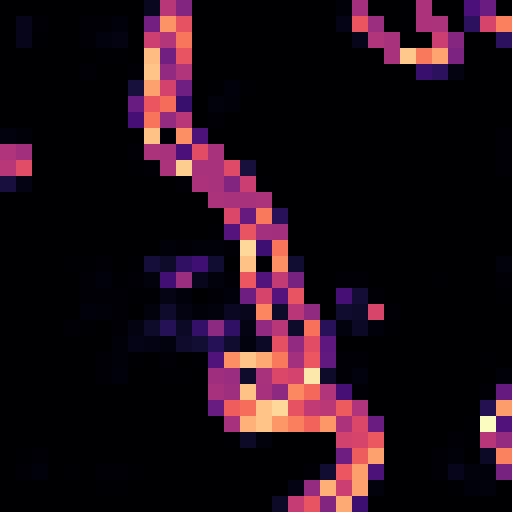
\includegraphics[width=1.0cm]{rasters/scene_tilephase.png}};
      \node[flat] (c4) at (1.7,-1.6) {
\includegraphics[width=1.0cm]{rasters/scene_ndwi.png}};
      \node[sub, below=0.6mm of c1] {boundary};
      \node[sub, below=0.6mm of c2] {low conf.};
      \node[sub, below=0.6mm of c3] {unstable};
      \node[sub, below=0.6mm of c4] {NDWI $\approx 0$};
    \end{tikzpicture}};
  \node[lab] at (4.6,2.35) {why each window};
  \draw[flow] (rev.west) -- (why.east);
  \draw[part, fill=oeviolet!15] (0.9,1.1) circle (0.33);
  \draw[part, fill=oeviolet!15] (0.35,-0.15) arc (180:0:0.55) -- cycle;
  \node[sub] at (0.9,-0.65) {reviewer / agent};
  \draw[flow] (why.west) -- (1.55,0.4);
\end{tikzpicture}
\end{document}
